% !TEX root = main_kpk_v01.tex
% !TEX program = pdflatex
% =====================================================================
% ICCSCI 2026 — Procedia Computer Science
% Paper: Detecting Corruption Indications in Village Fund Expenditure:
%        A Multi-Paradigm Unsupervised Machine Learning Approach
%        for Jambi Province, Indonesia
%
% Template: elsarticle + ecrc (Elsevier Procedia CRC)
% Citation style: Vancouver numbered [#]
% Double-blind submission — all author identities removed
%
% VERSION: main_kpk_v01.tex
%   - Tables 5 & 6 placed side-by-side (horizontal) in one table* float
%   - Prose condensed throughout; target 10 pages with references
%   - All substance, statistics, and arguments retained
% =====================================================================

\documentclass[3p,times,procedia]{elsarticle}
\flushbottom

%% ecrc package — required for Procedia CRC layout
\PassOptionsToPackage{procedia}{ecrc}
\usepackage{ecrc}
\usepackage[bookmarks=false]{hyperref}
    \hypersetup{colorlinks,
      linkcolor=blue,
      citecolor=blue,
      urlcolor=blue}

%% Core packages
\usepackage{graphicx}
\usepackage{stfloats}
\usepackage{amsmath}
\usepackage{amssymb}
\usepackage[figuresright]{rotating}

%% TikZ for research framework diagram
\usepackage{tikz}
\usetikzlibrary{arrows.meta, shapes.geometric, positioning, backgrounds, fit, calc}

\graphicspath{{../charts/}{../templates/}}

%% Journal metadata
\volume{00}
\firstpage{1}
\journalname{Procedia Computer Science}
\runauth{[BLINDED FOR REVIEW]}
\jid{procs}

% =====================================================================
\begin{document}
\begin{frontmatter}

\dochead{The 13th International Conference on Computer Science and Computational Intelligence (ICCSCI 2026)}

\title{Detecting Corruption Indications in Village Fund Expenditure: A Multi-Paradigm Unsupervised Machine Learning Approach for Jambi Province, Indonesia}

\author[a]{[Author~1~~~Blinded for Review]\corref{cor1}}
\author[b]{[Author~2~~~Blinded for Review]}
\address[a]{[Affiliation~1~~~Blinded for Review]}
\address[b]{[Affiliation~2~~~Blinded for Review]}
\cortext[cor1]{Corresponding author.}

\begin{abstract}
Indonesia's Dana Desa programme disburses approximately Rp~71 trillion annually to 75,259 villages, yet documented fraud spanning 640 defendants and Rp~598.13 billion in verified state losses reveals a persistent detection gap. Despite granular activity-level expenditure records maintained in Siskeudes, no automated pre-inspection screening mechanism operates at the provincial level. This study develops a three-method unsupervised machine learning pipeline---Isolation Forest (IF), Local Outlier Factor (LOF), and Robust Deep Autoencoder (RDA)---applied to 99,692 activity-level village fund expenditure records from Jambi Province across fiscal years 2023--2025, sourced via jaga.id. Seven typology-grounded features operationalize documented corruption modus operandi. A multi-paradigm consensus framework (agreement from $\geq$\,2 of 3 methods) identifies 3,107 high-confidence anomalous records (3.1\%). LOF achieves the highest bimodality coefficient (BC\,=\,0.957), demonstrating superior within-category anomaly discrimination. Consensus anomalies map predominantly to Mark-up (T1: 50.6\%) and Cross-Category Dump (T7: 50.5\%) typologies, consistent with judicial prosecution records. Village-level persistence analysis classifies 642 villages (47.1\%) as high-priority. The pipeline reduces the APIP inspection search space from 99,692 records to 642 priority villages---a 93.5\% reduction---without ground-truth labels, operationalising the DeLone and McLean IS Success Model for proactive anti-corruption triage.
\end{abstract}

\begin{keyword}
anomaly detection \sep village fund corruption \sep unsupervised machine learning \sep fraud detection \sep Dana Desa
\end{keyword}

\end{frontmatter}
\email{[email-blinded-for-review@institution.edu]}

\vspace*{-6pt}

% =====================================================================
\section{Introduction}
\label{sec:intro}

Indonesia's Dana Desa (Village Fund) programme represents one of the largest intergovernmental fiscal transfers in the developing world, channelling approximately Rp~71 trillion annually to 75,259 villages since the enactment of Law No.~6 of 2014 on Villages~\cite{ref1}. By 2024, Indonesian Corruption Watch (ICW) catalogued 591 court verdicts involving village fund misappropriation, implicating 640 defendants and documenting Rp~598.13 billion in verified state losses~\cite{ref2}. The Komisi Pemberantasan Korupsi (KPK) identified 851 village fund corruption cases from 2015 onward, with village heads accounting for more than 60\% of perpetrators~\cite{ref3}. These figures converge on a single diagnostic conclusion: the dominant response to village fund fraud remains reactive---prosecution occurring years after diversion---rather than proactive and data-driven.

The Sistem Keuangan Desa (Siskeudes), maintained by BPKP, records village fund expenditure at the activity level across each disbursement stage: planned activity type, budget allocation, realisation per tranche (T1, T2, T3), and procurement mechanism. This granular absorption data constitutes an administrative signal archive encoding, in latent form, financial patterns distinguishing legitimate from corrupt expenditure. Yet no systematic automated screening mechanism currently operates at the district or provincial level to interrogate this archive before inspection cycles conclude and disbursement windows close.

This detection gap persists despite KPK's Trisula prevention architecture~\cite{ref4} and four village-specific programmes: \textit{Desa Antikorupsi} (33 designated villages by 2024~\cite{ref5}), Siswaskeudes (adopted in only 105 of 504 kabupaten/kota~\cite{ref6}, with mandatory rollout pending under Stranas~PK 2025--2026~\cite{ref7}), the Monitoring Center for Prevention (MCP, operating at Pemda aggregate level~\cite{ref8}), and jaga.id (complaint-driven, structurally undercounting low-monitoring environments~\cite{ref9}). As Section~\ref{sec:kpk_prevention} details, none provides automated, activity-level pre-inspection screening at the record granularity Siskeudes maintains---the structural gap this study addresses.

Existing research concentrates on retrospective forensic analysis~\cite{ref10}, governance accountability frameworks~\cite{ref11}, and fraud triangle diagnostics~\cite{ref12}. Where machine learning enters the literature, it applies predominantly supervised classification---a paradigm requiring labelled ground truth unavailable in real-time monitoring contexts~\cite{ref13,ref14}. This study addresses that gap by developing an unsupervised pipeline that detects expenditure anomalies in Jambi Province's village fund records across FY~2023--2025 without pre-existing fraud labels.

Jambi Province provides a structurally significant research site. Throughout 2024--2026, jaga.id recorded only 11 complaint submissions attributed to Jambi (1.4\% of 761 national reports), while comparable provinces such as Sumatera Utara registered 81~\cite{ref9}. Low voluntary reporting signals a low-monitoring environment, not low fraud exposure: four contemporaneous Jambi prosecution cases document Rp~2.301 billion in verified losses across Kerinci, Muaro Jambi, and Tanjung Jabung Timur kabupaten~\cite{ref15,ref16,ref17,ref18}, with detection lags of two to five years. This study poses three research questions: (RQ1)~Which feature constructs derived from village fund absorption data discriminate corruption anomalies most effectively? (RQ2)~Which algorithm---IF, LOF, or RDA---demonstrates superior anomaly discrimination? (RQ3)~How do algorithmically identified anomalies map to established corruption typologies?

% =====================================================================
\section{Related Work}
\label{sec:related}

\subsection{Corruption Typology Frameworks}

Graycar's TASP framework demands that corruption analysis specify form, activity, sector, and context~\cite{ref19}. For the Dana Desa context, Siregar and Aminudin~\cite{ref13} provide the most relevant empirical classification: a multi-case analysis identifying five modus operandi---mark-up, fictitious budget items, double budgeting, procurement manipulation, and misuse of personnel funds. Kartadinata et al.~\cite{ref14} confirm mark-up (\textit{penggelembungan}) and fictitious projects (\textit{proyek fiktif}) as dominant patterns across 200$+$ KPK prosecution cases (2015--2020). Medan et al.~\cite{ref20} validate these modus operandi into 2025 in East Nusa Tenggara, confirming the continuing relevance of typology-grounded detection.

\subsection{Fraud Triangle and Principal-Agent Foundations}

Cressey's Fraud Triangle~\cite{ref21}, operationalised for the Dana Desa context by Hidajat~\cite{ref12}, models three conditions: Pressure (disbursement targets creating perverse incentives), Opportunity (structural absence of competitive procurement and limited auditor reach), and Rationalisation (normalisation of fund manipulation as low-risk). The 98.8\% Swakelola procurement dominance documented in the present dataset confirms S{\o}reide's~\cite{ref22} argument that absent competitive bidding is the primary structural enabler of procurement-stage corruption. Principal-agent theory~\cite{ref23} frames unexplained deviations from expected spending patterns as proximate evidence of information asymmetry exploitation---precisely the signal unsupervised anomaly detection targets.

\subsection{Anomaly Detection in Public Financial Data}

Three methodologically distinct paradigms operate as complements rather than substitutes. Isolation Forest (IF)~\cite{ref24,ref25} applies random partitioning path length as a global sparsity measure. Local Outlier Factor (LOF)~\cite{ref26} identifies records whose neighbourhood density differs from their $k$-nearest peers---an architecture that captures within-category price inflation structurally invisible to global methods. The Robust Deep Autoencoder (RDA)~\cite{ref27} augments autoencoder training with a sparse noise decomposition matrix, preventing anomalous records from corrupting the learned normal representation. Chandola et al.~\cite{ref28} establish that multi-paradigm approaches consistently outperform any single method. Prior work on Indonesian public financial data has not applied this three-paradigm ensemble to village fund activity-level records~\cite{ref29,ref30}.

\subsection{Information Systems Grounding}

The DeLone and McLean IS Success Model~\cite{ref31}---in its 2003 formulation---provides the IS-level justification for deploying an anomaly detection pipeline as an institutional intervention. Pipeline outputs (anomaly scores, typology labels, village priority tiers) constitute the Information Quality dimension, driving Individual Impact (auditor attention allocation) and Organisational Impact (corruption deterrence and state loss prevention). Mutungi et al.~\cite{ref11} demonstrate that digital anti-corruption tools fail when their design does not map to specific corruption interaction points---validating the typology-grounded feature engineering approach adopted here.

\subsection{KPK Prevention Architecture and Its Structural Gaps}
\label{sec:kpk_prevention}

KPK's Trisula strategy~\cite{ref4} positions prevention between education and enforcement. For 2025--2026, Stranas~PK designates village governance strengthening as one of 15 priority actions, recommending mandatory Siswaskeudes adoption and cross-ministerial data integration spanning Kemendes, Kemendagri, Kemenkeu, and Bappenas~\cite{ref7}.

The four village-specific programmes address distinct but non-overlapping corruption lifecycle segments. \textit{Desa Antikorupsi}~\cite{ref5} targets the Rationalisation dimension through community norm formation, reaching only 33 villages nationally by 2024. \textit{Siswaskeudes}~\cite{ref6} provides APIP with computer-assisted audit tools at the financial management process level but requires human inspector deployment and cannot generate ranked village priority lists autonomously. \textit{MCP}~\cite{ref8} monitors eight governance indicators at the kabupaten/kota aggregate level; its unit of analysis is the Pemda governance system, not individual Siskeudes activity records. \textit{jaga.id}~\cite{ref9} captures complaint-driven signals but structurally undercounts low-monitoring environments.

The detection gap is therefore one of \textit{granularity and automation}, not programme absence. Table~\ref{tab:kpk_comparison} maps these four instruments against the present pipeline across five dimensions, clarifying that the pipeline fills the activity-level automated pre-inspection screening slot the existing architecture structurally lacks---with outputs designed to feed directly into Siswaskeudes-equipped APIP inspectorates as pre-inspection intelligence.

\begin{table*}[htb]
\caption{Existing KPK prevention instruments vs.\ the present pipeline across five operational dimensions.}
\label{tab:kpk_comparison}
\begin{tabular*}{\hsize}{@{\extracolsep{\fill}}p{2.8cm}p{2.5cm}p{2.8cm}p{2.4cm}p{1.8cm}p{2.5cm}@{}}
\toprule
\textbf{Instrument} & \textbf{Operational Level} & \textbf{Detection Trigger} & \textbf{Coverage} & \textbf{Automation} & \textbf{Fraud Triangle Target} \\
\colrule
Desa Antikorupsi~\cite{ref5}  & Village           & Voluntary designation    & 33 villages (0.04\%)        & None    & Rationalisation \\
Siswaskeudes~\cite{ref6}       & Activity record   & Human APIP inspection    & 105/504 kabupaten           & Partial (TABK) & Opportunity \\
MCP~\cite{ref8}                & Kabupaten/kota    & Annual governance scoring & 546 Pemda (2023)            & Partial & Opportunity \\
jaga.id~\cite{ref9}            & Village           & Community complaint      & 761 national reports        & None    & All (reactive) \\
\textbf{This pipeline}         & \textbf{Activity record}  & \textbf{Automated anomaly scoring} & \textbf{All 1,364 Jambi villages} & \textbf{Full} & \textbf{All (proactive)} \\
\botrule
\end{tabular*}
\end{table*}

% =====================================================================
\section{Methodology}
\label{sec:method}

Fig.~\ref{fig:framework} presents the complete end-to-end pipeline: six processing layers from jaga.id data acquisition through feature construction, three-paradigm detection, multi-method consensus, typology assignment, and APIP inspection workplan generation---with theoretical grounding from the Fraud Triangle, Principal-Agent Theory, and DeLone \& McLean IS Success Model.

\begin{figure*}[htb]
\centering
\resizebox{\textwidth}{!}{%
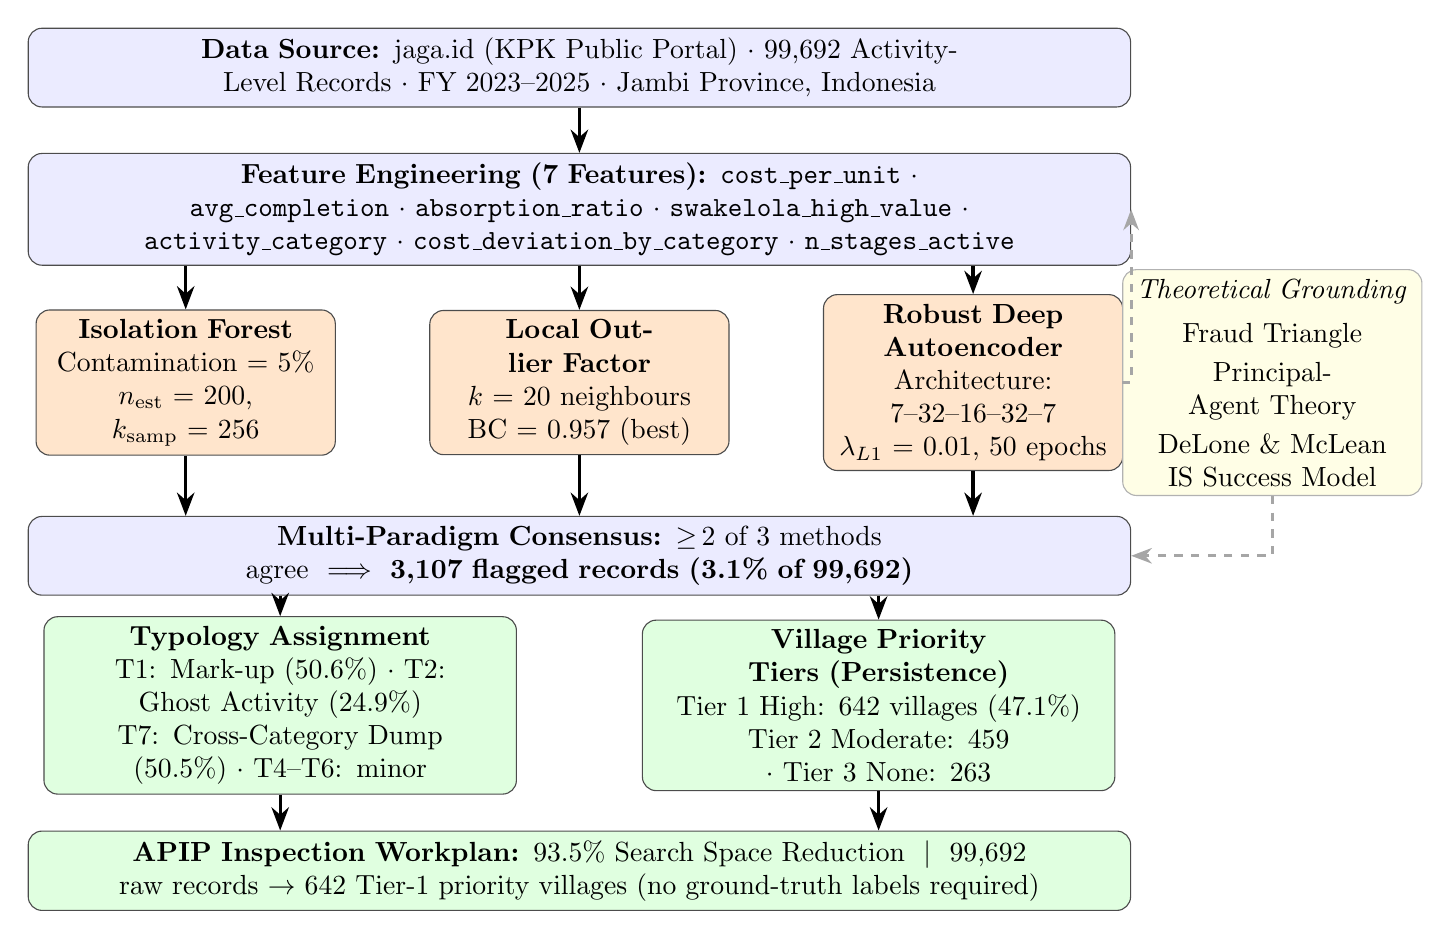
\begin{tikzpicture}[
  box/.style={rectangle, rounded corners=5pt, draw=black!70, fill=blue!8,
              text centered, minimum height=1.0cm, font=\normalsize},
  algo/.style={rectangle, rounded corners=5pt, draw=black!70, fill=orange!20,
               text centered, minimum height=1.0cm, font=\normalsize},
  outbox/.style={rectangle, rounded corners=5pt, draw=black!70, fill=green!12,
                 text centered, minimum height=1.0cm, font=\normalsize},
  thbox/.style={rectangle, rounded corners=5pt, draw=gray!60, fill=yellow!10,
                text centered, minimum height=1.0cm, font=\normalsize, align=center},
  arr/.style={->, >=Stealth, line width=1.2pt},
  darr/.style={->, >=Stealth, dashed, gray!70, line width=1pt}]

  \node[box, minimum width=14cm, text width=13.5cm] at (0, 0) (data)
    {\textbf{Data Source:} jaga.id (KPK Public Portal) $\cdot$ 99,692 Activity-Level Records $\cdot$ FY 2023--2025 $\cdot$ Jambi Province, Indonesia};

  \node[box, minimum width=14cm, text width=13.5cm] at (0, -1.8) (feat)
    {\textbf{Feature Engineering (7 Features):} \texttt{cost\_per\_unit} $\cdot$ \texttt{avg\_completion} $\cdot$ \texttt{absorption\_ratio} $\cdot$ \texttt{swakelola\_high\_value} $\cdot$ \texttt{activity\_category} $\cdot$ \texttt{cost\_deviation\_by\_category} $\cdot$ \texttt{n\_stages\_active}};

  \node[algo, minimum width=3.8cm, text width=3.5cm, align=center] at (-5.0, -4.0) (if)
    {\textbf{Isolation Forest}\\Contamination = 5\%\\$n_{\text{est}}$ = 200, $k_{\text{samp}}$ = 256};

  \node[algo, minimum width=3.8cm, text width=3.5cm, align=center] at (0, -4.0) (lof)
    {\textbf{Local Outlier Factor}\\$k$ = 20 neighbours\\BC = 0.957 (best)};

  \node[algo, minimum width=3.8cm, text width=3.5cm, align=center] at (5.0, -4.0) (rda)
    {\textbf{Robust Deep Autoencoder}\\Architecture: 7--32--16--32--7\\ $\lambda_{L1}$ = 0.01, 50 epochs};

  \node[box, minimum width=14cm, text width=13.5cm] at (0, -6.2) (cons)
    {\textbf{Multi-Paradigm Consensus:} $\geq$\,2 of 3 methods agree $\ \Longrightarrow\ $ \textbf{3,107 flagged records (3.1\% of 99,692)}};

  \node[outbox, minimum width=6.0cm, text width=5.7cm, align=center] at (-3.8, -8.1) (typo)
    {\textbf{Typology Assignment}\\T1: Mark-up (50.6\%) $\cdot$ T2: Ghost Activity (24.9\%)\\T7: Cross-Category Dump (50.5\%) $\cdot$ T4--T6: minor};

  \node[outbox, minimum width=6.0cm, text width=5.7cm, align=center] at (3.8, -8.1) (vil)
    {\textbf{Village Priority Tiers (Persistence)}\\Tier 1 High: 642 villages (47.1\%)\\Tier 2 Moderate: 459 $\cdot$ Tier 3 None: 263};

  \node[outbox, minimum width=14cm, text width=13.5cm] at (0, -10.2) (work)
    {\textbf{APIP Inspection Workplan:} 93.5\% Search Space Reduction $\ |\ $ 99,692 raw records $\rightarrow$ 642 Tier-1 priority villages (no ground-truth labels required)};

  \node[thbox, minimum width=3.8cm, text width=3.5cm] at (8.8, -4.0) (theory)
    {\textit{Theoretical Grounding}\\[4pt]
     Fraud Triangle\\[2pt]
     Principal-Agent Theory\\[2pt]
     DeLone \& McLean\\IS Success Model};

  \draw[arr] (data.south)             -- (feat.north);
  \draw[arr] (feat.south -| if)       -- (if.north);
  \draw[arr] (feat.south)             -- (lof.north);
  \draw[arr] (feat.south -| rda)      -- (rda.north);
  \draw[arr] (if.south)               -- (cons.north -| if);
  \draw[arr] (lof.south)              -- (cons.north);
  \draw[arr] (rda.south)              -- (cons.north -| rda);
  \draw[arr] (cons.south -| typo)     -- (typo.north);
  \draw[arr] (cons.south -| vil)      -- (vil.north);
  \draw[arr] (typo.south) -- ++(0,-0.4) -| (work.north -| typo);
  \draw[arr] (vil.south)  -- ++(0,-0.4) -| (work.north -| vil);
  \draw[darr] (theory.west)  -| (feat.east);
  \draw[darr] (theory.south) |- (cons.east);

\end{tikzpicture}}
\caption{Research framework: from jaga.id data collection through multi-paradigm unsupervised anomaly detection to APIP inspection workplan. Theoretical grounding integrates Fraud Triangle~\cite{ref21}, Principal-Agent Theory~\cite{ref23}, and DeLone \& McLean IS Success Model~\cite{ref31}.}
\label{fig:framework}
\end{figure*}

\subsection{Dataset and Data Sources}

The study uses activity-level village fund expenditure records collected via jaga.id (\url{https://jaga.id})---the KPK-operated public monitoring portal providing open access to village fund expenditure realization records at the provincial level~\cite{ref9}. Two complementary sources were merged via composite key \texttt{Kode\_Desa} $\times$ \texttt{Tahun}: (1)~\textit{Penyerapan} (expenditure absorption) records documenting realised spending per activity per disbursement stage, and (2)~\textit{Pagu} (budget ceiling) records documenting approved allocations. The final longitudinal panel contains \textbf{99,692 activity-level records} (33,140 in 2023; 36,151 in 2024; 30,401 in 2025), covering all kabupaten/kota in Jambi Province. No pre-existing fraud labels attach to any record; detection is entirely unsupervised.

\subsection{Feature Engineering}
\label{sec:features}

Seven features were engineered to operationalise corruption modus operandi documented in judicial records and institutional audit reports~\cite{ref13,ref14}. Table~\ref{tab:features} lists construction rules and targeted modus operandi. All continuous features were standardised (zero mean, unit variance) prior to model input.

\begin{table*}[htb]
\caption{Engineered features and corresponding corruption modus operandi.}
\label{tab:features}
\begin{tabular*}{\hsize}{@{\extracolsep{\fill}}llp{4.5cm}@{}}
\toprule
\textbf{Feature} & \textbf{Construction} & \textbf{Modus Operandi Targeted} \\
\colrule
\texttt{cost\_per\_unit}            & Total realisation $\div$ Volume (normalised)                   & Mark-up / price inflation \\
\texttt{absorption\_ratio}          & Total realisation $\div$ Pagu (village-level)                  & Ghost activity (near-zero absorption) \\
\texttt{avg\_completion}            & Mean(Pct\_T1, Pct\_T2, Pct\_T3)                               & Manipulated completion reporting \\
\texttt{swakelola\_high\_value}     & Binary: Swakelola AND realisation above threshold              & High-value uncompetitive procurement \\
\texttt{activity\_category}         & \texttt{Kode\_Output} 2-digit prefix (ordinally encoded)       & Cross-category activity mismatch \\
\texttt{cost\_deviation\_by\_category} & $z$-score of \texttt{cost\_per\_unit} within \texttt{Kode\_Output} group & Within-category price outlier \\
\texttt{n\_stages\_active}          & Count of disbursement stages with Real $> 0$                   & Incomplete / front-loaded disbursement \\
\botrule
\end{tabular*}
\end{table*}

Fig.~\ref{fig:feat_dist} presents raw feature distributions and the inter-feature correlation structure.

\begin{figure*}[htb]
\centering
\begin{minipage}[t]{0.61\textwidth}
  \centering
  
\includegraphics[width=\linewidth]{feature_distributions.png}\\[2pt]
  {\small\textbf{(a)}}
\end{minipage}\hfill
\begin{minipage}[t]{0.37\textwidth}
  \centering
  
\includegraphics[width=\linewidth]{feature_correlation_heatmap.png}\\[2pt]
  {\small\textbf{(b)}}
\end{minipage}
\caption{\textbf{(a)} Feature distributions across all 99,692 records (clipped at 99th percentile). Extreme right-skew in \texttt{cost\_per\_unit} (median = Rp~5,440,000; max = Rp~$2.8{\times}10^8$) and near-binary concentration in \texttt{absorption\_ratio} (median = 0.02) are consistent with incomplete fund absorption patterns.
\textbf{(b)} Pairwise feature correlation matrix (Pearson $r$). Strongest correlation: \texttt{cost\_deviation\_by\_category} $\leftrightarrow$ \texttt{cost\_per\_unit} ($r = 0.59$); all other pairs $|r| < 0.40$, confirming sufficient feature independence for multi-method detection.}
\label{fig:feat_dist}%
\label{fig:feat_corr}
\end{figure*}

\subsection{Detection Algorithms}

\textbf{Isolation Forest (IF)} partitions the feature space via random axis-aligned splits~\cite{ref24,ref25}. Records requiring fewer partitions to isolate receive lower anomaly scores. Contamination = 5\%; $n_{\text{estimators}} = 200$; $\texttt{max\_samples} = 256$; $\texttt{random\_state} = 42$.

\textbf{Local Outlier Factor (LOF)} computes for each record the ratio of its estimated local reachability density to the mean local reachability density of its $k$-nearest neighbours~\cite{ref26}. Records with LOF $\gg 1.0$ are locally dense isolates. $n_{\text{neighbors}} = 20$; full-training evaluation (\texttt{novelty = False}).

\textbf{Robust Deep Autoencoder (RDA)} decomposes input matrix $\mathbf{X}$ into a learned normal representation $\mathbf{L}$ and a sparse noise matrix $\mathbf{S}$ ($L_1$-penalised), preventing anomalous records from corrupting the learned representation~\cite{ref27}. Anomaly scores are mean squared error between input and reconstruction. Architecture: $[7 \to 32 \to 16 \to 32 \to 7]$, ReLU activations; epochs = 50; batch size = 256; $\lambda_{L1} = 0.01$.

\subsection{Consensus Framework and Typology Mapping}

A record receives \texttt{consensus\_flag = 1} if flagged by $\geq$\,2 of 3 methods. Consensus-flagged records are post-processed through a rule-based typology module mapping feature profiles to seven typology labels (T1--T7). The schema synthesises three empirical sources: Siregar and Aminudin's modus operandi taxonomy~\cite{ref13}, Kartadinata et al.'s systematic classification of 200$+$ KPK prosecution cases~\cite{ref14}, and Hidajat's anti-corruption mode analysis~\cite{ref12}. Table~\ref{tab:typo_rules} presents the full feature-to-typology assignment rules. Records satisfying no individual rule threshold receive an \textit{Unclassified} assignment.

\begin{table*}[htb]
\caption{Corruption typology assignment rules for consensus-flagged records. Schema derived from triangulation of~\cite{ref12,ref13,ref14}.}
\label{tab:typo_rules}
\begin{tabular*}{\hsize}{@{\extracolsep{\fill}}cll@{}}
\toprule
\textbf{Code} & \textbf{Typology} & \textbf{Primary Feature Signal} \\
\colrule
T1 & Mark-up / Price Inflation   & \texttt{cost\_per\_unit} $> 3\sigma$ AND \texttt{cost\_deviation\_by\_category} $> 2\sigma$ \\
T2 & Ghost Activity              & \texttt{absorption\_ratio} $< 0.05$ AND \texttt{avg\_completion} $< 10\%$ \\
T3 & Volume Padding              & \texttt{n\_stages\_active} = 1, \texttt{cost\_per\_unit} within normal range \\
T4 & Stage Lock                  & \texttt{n\_stages\_active} = 0 (budget allocated, zero disbursement) \\
T5 & Procurement Irregularity    & \texttt{swakelola\_high\_value} = 1 AND \texttt{cost\_per\_unit} $> 5\sigma$ \\
T6 & Budget Exhaustion           & \texttt{absorption\_ratio} $> 0.98$ AND \texttt{avg\_completion} $< 50\%$ \\
T7 & Cross-Category Dump         & \texttt{activity\_category} mismatch relative to \texttt{Kode\_Output} peer group \\
\botrule
\end{tabular*}
\end{table*}

\subsection{Village Priority Tier Classification}

Village-level priority tiers aggregate activity-level consensus flags into an anomaly persistence score per village across three fiscal years: Tier~1 (High Priority) for flags in $\geq$\,2 years; Tier~2 (Moderate) for flags in exactly 1 year; Tier~3 (Not Flagged) for none. Multi-year persistence operationalises the Opportunity condition of the Fraud Triangle~\cite{ref21}: recurrence signals entrenched structural vulnerability rather than incidental deviation.

% =====================================================================
\section{Results}
\label{sec:results}

\subsection{Per-Method Anomaly Detection Rates}

Table~\ref{tab:rates} presents anomaly flag counts and detection rates per method across fiscal years. Fig.~\ref{fig:rate_consist} visualises cross-year rate consistency.

\begin{table}[htb]
\caption{Per-method anomaly flag counts and detection rates.}
\label{tab:rates}
\begin{tabular*}{\hsize}{@{\extracolsep{\fill}}lrrrrr@{}}
\toprule
\textbf{Method} & \textbf{Total} & \textbf{Overall} & \textbf{2023} & \textbf{2024} & \textbf{2025} \\
\colrule
IQR Baseline          & 18,478 & 18.5\% & 21.1\% & 17.6\% & 17.1\% \\
Isolation Forest (IF) &  7,974 &  8.0\% & 10.5\% &  6.5\% &  7.1\% \\
LOF                   &  4,985 &  5.0\% &  4.7\% &  4.6\% &  5.8\% \\
RDA (Dense AE)        &  4,985 &  5.0\% &  5.5\% &  3.8\% &  5.9\% \\
\textbf{Consensus ($\geq$2/3)} & \textbf{3,107} & \textbf{3.1\%} & 4.1\% & 2.0\% & 3.3\% \\
\botrule
\end{tabular*}
\end{table}

\begin{figure*}[htb]
\centering

\includegraphics[width=0.74\textwidth]{anomaly_rate_consistency.png}
\caption{Anomaly rate consistency per method and fiscal year. LOF exhibits the most stable cross-year profile (range: 4.6--5.8\%); Isolation Forest shows the highest inter-year variance (10.5\% in 2023 vs.\ 6.5\% in 2024), reflecting post-COVID fiscal expansion dynamics.}
\label{fig:rate_consist}
\end{figure*}

\subsection{Score Distributions and Inter-Method Agreement}

Fig.~\ref{fig:score_dist} presents score distribution histograms annotated with Bimodality Coefficient (BC) values, where BC $> 0.555$ indicates bimodal separation between the normal cluster and the anomaly tail.

\begin{figure*}[htb]
\centering

\includegraphics[width=0.74\textwidth]{score_distributions.png}
\caption{Score distribution histograms for all three methods. LOF (BC = 0.957) exhibits a sharply L-shaped distribution; RDA (BC = 0.703) confirms a clear anomaly tail; IF (BC = 0.335) is unimodal---its 95th-percentile threshold cuts through a high-density score region.}
\label{fig:score_dist}
\end{figure*}

Tables~\ref{tab:bc} and~\ref{tab:overlap} summarise bimodality coefficients and pairwise flag overlap. IF and RDA converge on 50.3\% of RDA's flagged records---both respond to globally extreme multi-feature deviations (\texttt{cost\_per\_unit} at 102.83$\sigma$; \texttt{cost\_deviation\_by\_category} at 42.42$\sigma$). LOF's low overlap with both methods (6.4\% with IF; 12.0\% with RDA) confirms that LOF identifies a structurally distinct anomaly subset through its local density architecture. The 156 triple-consensus records constitute the highest-confidence fraud signals.

%% Tables 5 & 6 placed side-by-side horizontally inside one table* float
\begin{table*}[htb]
\begin{minipage}[t]{0.46\textwidth}
\caption{Bimodality coefficient and score range per method.}
\label{tab:bc}
\begin{tabular*}{\linewidth}{@{\extracolsep{\fill}}lcp{2.8cm}@{}}
\toprule
\textbf{Method} & \textbf{BC} & \textbf{Interpretation} \\
\colrule
Isolation Forest  & 0.335 & Unimodal---no clean separation \\
RDA               & 0.703 & Moderate bimodal---clear anomaly tail \\
\textbf{LOF}      & \textbf{0.957} & \textbf{Strong bimodal---sharpest discrimination} \\
\botrule
\end{tabular*}
\end{minipage}\hfill
\begin{minipage}[t]{0.50\textwidth}
\caption{Pairwise flag overlap between detection methods.}
\label{tab:overlap}
\begin{tabular*}{\linewidth}{@{\extracolsep{\fill}}lrr@{}}
\toprule
\textbf{Method Pair} & \textbf{Records in Both} & \textbf{\% of Smaller Method} \\
\colrule
IF $\cap$ LOF              &   317 &  6.4\% \\
IF $\cap$ RDA              & 2,506 & \textbf{50.3\%} \\
LOF $\cap$ RDA             &   596 & 12.0\% \\
IF $\cap$ LOF $\cap$ RDA (triple) & 156 & 1.6\% of total \\
\botrule
\end{tabular*}
\end{minipage}
\end{table*}

\subsection{Corruption Typology Distribution}

Fig.~\ref{fig:typology} and Table~\ref{tab:typology} present typology distribution among consensus-flagged records using multi-label assignment (a record may satisfy multiple typology rules simultaneously).

\begin{figure*}[htb]
\centering
\begin{minipage}[t]{0.63\textwidth}
  \centering
  
\includegraphics[width=\linewidth]{typology_distribution.png}\\[2pt]
  {\small\textbf{(a)}}
\end{minipage}\hfill
\begin{minipage}[t]{0.34\textwidth}
  \centering
  
\includegraphics[width=\linewidth]{village_persistence_tiers.png}\\[2pt]
  {\small\textbf{(b)}}
\end{minipage}
\caption{\textbf{(a)} Corruption typology distribution among 3,107 consensus-flagged records (multi-label). T1 (Mark-up) and T7 (Cross-Category Dump) co-dominate at 50.6\% and 50.5\%. T4 (Stage Lock) registers zero detections---a subthreshold masking pattern discussed in Section~\ref{sec:discussion}.
\textbf{(b)} Village priority tier distribution based on anomaly persistence across FY~2023--2025. Tier~1 (642 villages, 47.1\%) exhibit consensus flags in $\geq$\,2 fiscal years, indicating entrenched structural vulnerability.}
\label{fig:typology}%
\label{fig:village_tiers}
\end{figure*}

\begin{table}[htb]
\caption{Corruption typology frequencies (multi-label, consensus-flagged records, $n = 3{,}107$).}
\label{tab:typology}
\begin{tabular*}{\hsize}{@{\extracolsep{\fill}}clrr@{}}
\toprule
\textbf{Code} & \textbf{Typology} & \textbf{Count} & \textbf{\% Flagged} \\
\colrule
T1  & Mark-up / Price Inflation  & 1,571 & 50.6\% \\
T2  & Ghost Activity             &   774 & 24.9\% \\
T3  & Volume Padding             &    38 &  1.2\% \\
T4  & Stage Lock                 &     0 &  0.0\% \\
T5  & Procurement Irregularity   &    26 &  0.8\% \\
T6  & Budget Exhaustion          &    32 &  1.0\% \\
T7  & Cross-Category Dump        & 1,568 & 50.5\% \\
--- & Unclassified               &   708 & 22.8\% \\
\botrule
\end{tabular*}
\end{table}

\subsection{RDA Feature Importance, Village Tiers, and Spatial Projection}

Fig.~\ref{fig:rda_error} decomposes RDA reconstruction error by feature across all consensus-flagged records. \texttt{avg\_completion} dominates reconstruction error (MSE $\approx$ 0.00145), confirming that completion percentage manipulation generates the largest departure from learned normal fund absorption behaviour; \texttt{cost\_per\_unit} ranks second (MSE $\approx$ 0.00095). Of 1,364 unique villages, 642~(47.1\%) qualify as Tier~1 (High Priority)---exhibiting consensus anomalies in two or more fiscal years. This distribution, with nearly half of all villages showing multi-year persistence, is inconsistent with incidental error and indicates systemic, structurally sustained irregular spending. Fig.~\ref{fig:pca} confirms separability structure in the engineered feature space through PCA and t-SNE dimensionality reduction.

\begin{figure*}[htb]
\centering

\includegraphics[width=0.78\textwidth]{rda_error_decomposition.png}
\caption{Left: Mean RDA reconstruction error per feature across all consensus-flagged records. \texttt{avg\_completion} dominates (MSE $\approx 0.00145$), followed by \texttt{cost\_per\_unit} and \texttt{activity\_category}. Right: Per-record error heatmap for top-50 flagged records. The extreme outlier shows near-maximum error on both features---a compound fraud signature consistent with simultaneous price inflation and completion falsification.}
\label{fig:rda_error}
\end{figure*}

\begin{figure*}[htb]
\centering
\begin{minipage}[t]{0.49\textwidth}
  \centering
  
\includegraphics[width=\linewidth]{pca_projection.png}\\[2pt]
  {\small\textbf{(a)}}
\end{minipage}\hfill
\begin{minipage}[t]{0.49\textwidth}
  \centering
  
\includegraphics[width=\linewidth]{tsne_projection.png}\\[2pt]
  {\small\textbf{(b)}}
\end{minipage}
\caption{\textbf{(a)} PCA projection (PC1 = 26.0\%, PC2 = 12.7\% variance). Consensus anomalies ($n = 3{,}107$, red) distribute along the positive PC1 gradient; extreme outliers reach PC1 $> 40$.
\textbf{(b)} t-SNE projection (sampled: 14,538 normal + 462 anomalous). Anomaly concentration in specific right-periphery sub-clusters confirms systematic repetition of corruption patterns within programme category neighbourhoods, not random individual deviation.}
\label{fig:pca}%
\label{fig:tsne}
\end{figure*}

% =====================================================================
\section{Discussion}
\label{sec:discussion}

\subsection{Algorithm Selection: LOF's Superiority Is Theoretically Predicted}

LOF's bimodality coefficient of 0.957 is a theoretically predictable consequence of how corruption manifests structurally in Siskeudes records. Village fund activities within the same \texttt{Kode\_Output} prefix form natural local density clusters---road construction, PAUD operations, and BLT disbursements share characteristic cost ranges, procurement types, and stage structures. When a fraudulent record occupies such a cluster at 42.42 standard deviations above its category mean, LOF correctly identifies it as a local outlier even when IF's path-partitioning finds it globally unremarkable~\cite{ref26}. IF's unimodal score distribution (BC = 0.335) reflects structural misalignment: village fund corruption clusters by activity type rather than as globally random sparsity, suppressing the score variance IF requires for bimodal separation. The consensus framework resolves this heterogeneity---the IF $\cap$ RDA intersection (50.3\%, $n = 2{,}506$) captures globally extreme anomalies confirmed by two independent global paradigms; the LOF-unique population captures within-category deviants; the 156 triple-consensus records represent highest-confidence signals across all modalities. An APIP system relying solely on IF would structurally miss the locally deviant activities whose cost structure is abnormal relative to their programme category but unremarkable in the global distribution.

\subsection{Fraud Triangle in the Data}

All three conditions find quantitative expression in the results. \textit{Pressure} manifests in IF's elevated 2023 anomaly rate (10.5\% versus 6.5--7.1\% in subsequent years), coinciding with post-COVID village budget expansion when disbursement targets created stronger incentives for inflated claims. \textit{Opportunity} is confirmed by 98.8\% Swakelola procurement dominance---the structural condition S{\o}reide~\cite{ref22} identifies as the primary enabler: self-managed activities face no competitive bidding, no independent price verification, and no pre-disbursement external audit. The 642 Tier-1 villages (47.1\%) demonstrating multi-year persistence confirm entrenched rather than incidental opportunity---the same villages display irregular patterns across consecutive fiscal years. \textit{Rationalisation} leaves its imprint in the typology distribution: T1 ($n = 1{,}571$) and T7 ($n = 1{,}568$) dominate over operationally complex schemes (T3 = 38; T5 = 26), consistent with actors preferring administratively ambiguous patterns perceived as low-detection-risk~\cite{ref21}. The comparative rarity of T2 Ghost Activity ($n = 774$) relative to T1/T7 suggests perpetrators prefer documentation ambiguity over systematic project falsification.

\subsection{Principal-Agent Asymmetry, Subthreshold Masking, and Audit Intelligence}

The dominant RDA error feature---\texttt{avg\_completion}---locates precisely where information asymmetry operates with greatest consequence~\cite{ref23}. Village heads report T1 disbursement near 100\% while T2 and T3 stage realisations approach zero---a tranche progression pattern the autoencoder reconstructs with maximum error (MSE $\approx$ 0.00145) because no legitimate absorption behaviour produces this profile. This exploitation is possible because APIP inspection cycles typically conclude after T3 disbursement windows close. The RDA decomposition advises reversing the conventional APIP inspection sequence: cross-checking reported completion percentages against field evidence of physical output should precede procurement documentation review, since the completion reporting channel is where document-level manipulation is most feasible without physical corroboration.

The 708 unclassified consensus records (22.8\%) warrant explicit attention beyond classification residual treatment. These records satisfy the multi-paradigm threshold---confirmed anomalous by $\geq$\,2 independent methods---yet fail every individual typology rule threshold. The most plausible explanation is compound fraud: schemes combining moderate mark-up with partial completion manipulation such that no single feature exceeds its individual threshold while the joint profile remains statistically anomalous. For APIP, these records require full inter-feature intelligence---cross-referencing completion, cost, and category dimensions simultaneously---and should be prioritised for in-depth desk review before any field visit assignment.

\subsection{DeLone and McLean Evaluation and Institutional Positioning}

The DeLone and McLean model~\cite{ref31} evaluates three dimensions. \textit{Information Quality}: consensus scores, typology labels, and priority tiers are validated by multi-paradigm convergence, alignment with documented judicial modus operandi~\cite{ref13,ref14}, and the four Jambi prosecution cases confirming targeted financial patterns in verified fraud~\cite{ref15,ref16,ref17,ref18}. \textit{Individual Impact}: the ranked priority list reduces APIP's search space by 93.5\%, directly addressing the staffing constraint documented by Srirejeki and Faturokhman~\cite{ref29}. \textit{Organisational Impact}: realising this impact requires APIP inspectorates to institutionalise pipeline outputs as formal pre-inspection intelligence---a governance design challenge requiring procedure amendments and inspector training.

The pipeline's institutional positioning is most clearly understood by mapping it against the prevention gap KPK's own diagnosis identifies: the two-to-five-year detection lag in Jambi prosecution cases~\cite{ref15,ref16,ref17,ref18} reveals that the Trisula prevention channel~\cite{ref4} lacks activity-level automated screening within the fiscal year of expenditure realisation. Where Siswaskeudes is deployed~\cite{ref6}, typology-labelled outputs integrate directly with TABK workflows as a pre-prioritisation filter; where adoption is absent, outputs constitute the primary automated screening layer and support the Siswaskeudes adoption business case. MCP's Tata Kelola Dana Desa governance scoring~\cite{ref8} measures input and process indicators; the pipeline measures output indicators---a kabupaten with high MCP score yet high Tier-1 village concentration signals procedural compliance diverging from substantive outcome, a diagnostic signal in itself. For \textit{Desa Antikorupsi}~\cite{ref5}, the 263 Tier-3 villages (19.3\%) demonstrating three consecutive anomaly-free fiscal years provide an empirically grounded designation candidate pool, transforming a coverage-constrained programme (33 villages nationally) into a scalable accountability recognition mechanism grounded in Siskeudes absorption evidence.

% =====================================================================
\section{Conclusion}
\label{sec:conclusion}

This study develops and evaluates a comparative unsupervised machine learning pipeline applied to 99,692 activity-level village fund expenditure records from Jambi Province (FY~2023--2025). Three research questions were answered empirically.

\textbf{RQ1}: Seven engineered features operationalising documented corruption modus operandi~\cite{ref13,ref14} produce sufficient discriminating power without pre-existing fraud labels. RDA reconstruction error identifies \texttt{avg\_completion} as the dominant corruption signal (MSE $\approx$ 0.00145), followed by \texttt{cost\_per\_unit} and \texttt{activity\_category}. Extreme right-skew in \texttt{cost\_per\_unit} (max $= 102.83\sigma$) and \texttt{cost\_deviation\_by\_category} (max $= 42.42\sigma$) confirms that price inflation leaves detectable quantitative traces in Siskeudes absorption records without judicial corroboration.

\textbf{RQ2}: LOF achieves the highest bimodality coefficient (BC = 0.957)---superiority theoretically predicted by its local density architecture operating on within-category peer groups, where global methods (IF: BC = 0.335; RDA: BC = 0.703) are structurally blind. The multi-paradigm consensus aggregates complementary detection channels into 3,107 high-confidence flagged records that no single algorithm produces independently.

\textbf{RQ3}: Consensus anomalies map predominantly to T1 (Mark-up, 50.6\%) and T7 (Cross-Category Dump, 50.5\%), consistent with Jambi judicial records~\cite{ref15,ref16,ref17,ref18} and prior typology studies~\cite{ref13,ref14}. The 708 unclassified records (22.8\%)---multi-method confirmed but single-feature subthreshold---represent the methodologically most challenging class, requiring inter-feature combined analysis rather than single-indicator examination.

The pipeline operationalises the DeLone and McLean information-quality-to-organisational-impact pathway~\cite{ref31} by reducing APIP's search space from 99,692 records to 642 priority villages (93.5\% reduction) without pre-existing labels. Typology-labelled outputs---mark-up amounts, cross-category budget migration profiles, and stage-completion inconsistencies---can support KPK and Kejaksaan preliminary inquiry targeting, potentially reducing the two-to-five-year detection lag documented in Jambi prosecution cases~\cite{ref15,ref16,ref17,ref18}. The pipeline fills the automated, activity-level screening slot the existing prevention architecture structurally lacks~\cite{ref7}: its Tier-1 output feeds Siswaskeudes TABK prioritisation~\cite{ref6}; its Tier-3 output provides evidence for data-driven \textit{Desa Antikorupsi} designation~\cite{ref5}; and its typology labels support preliminary inquiry within the fiscal year of expenditure realisation, strengthening the Trisula prevention channel~\cite{ref4} at the granularity level where the existing instruments are absent.

\textbf{Limitations}: (1)~Single-province scope limits generalisability to provinces with structurally different disbursement patterns. (2)~jaga.id data derives from village-entered Siskeudes records; systematic misreporting at entry constitutes an undetectable data quality risk. (3)~Ground-truth labels are unavailable at the activity level, preventing precision--recall evaluation. (4)~The 5\% IF contamination rate is an unverified prior; miscalibration shifts the decision boundary into high-density score regions. (5)~Single-threshold typology rules cannot capture compound fraud at moderate but jointly anomalous multi-feature deviations. (6)~LOF's $O(n^2)$ complexity limits scalability beyond $\sim$100k records without approximate search optimisation.

\textbf{Future directions}: (1)~Match pipeline-flagged activities against KPK/Kejaksaan prosecution indictments to build annotated training data and calibrate typology classification accuracy empirically. (2)~Fuse SP2D (Kemendagri) and OM-SPAN (Kemenkeu) records with jaga.id absorption figures as cross-validation layers, reducing single-source data quality risk. (3)~Calibrate contamination rates using expert-annotated APIP inspection samples. (4)~Extend to the FY~2018--2025 longitudinal panel to improve persistence detection reliability and model corruption pattern evolution across dana desa programme maturation phases.

% =====================================================================
%% References — Vancouver numbered style, ordered by appearance
% =====================================================================
\begin{thebibliography}{46}

\bibitem{ref1}
Republic of Indonesia. Undang-Undang Nomor 6 Tahun 2014 tentang Desa [Law No.~6 of 2014 on Villages]. Jakarta; 2014.

\bibitem{ref2}
Indonesian Corruption Watch (ICW). Laporan Tren Penindakan Kasus Korupsi Dana Desa 2024. Jakarta: ICW; 2024. Available: \url{https://antikorupsi.org}

\bibitem{ref3}
Komisi Pemberantasan Korupsi (KPK). Statistik Perkara Korupsi Dana Desa 2015--2024. Jakarta: KPK; 2024. Available: \url{https://www.kpk.go.id}

\bibitem{ref4}
Komisi Pemberantasan Korupsi (KPK). Trisula Strategi Pemberantasan Korupsi: Pendidikan, Pencegahan, dan Penindakan. Jakarta: KPK; 2022. Available: \url{https://aclc.kpk.go.id/aksi-informasi/Eksplorasi/20220511-trisula-strategi-pemberantasan-korupsi-kpk-untuk-visi-indonesia-bebas-dari-korupsi}

\bibitem{ref5}
Komisi Pemberantasan Korupsi (KPK). Pendidikan dan Pencegahan Korupsi di Tingkat Desa: Program Desa Antikorupsi 2021--2024. Jakarta: KPK; 2025. Available: \url{https://kpk.go.id/id/ruang-informasi/berita/pendidikan-dan-pencegahan-korupsi-di-tingkat-desa}

\bibitem{ref6}
Setnas Pencegahan Korupsi / KPK. Capaian Pengawasan Keuangan Desa: Implementasi Siswaskeudes di Kabupaten/Kota. Jakarta: Stranas~PK; 2020. Available: \url{https://stranaspk.kpk.go.id/id/berita/capaian-pengawasan-keuangan-desa-pada-triwulan-vi}

\bibitem{ref7}
Komisi Pemberantasan Korupsi (KPK). Stranas~PK Luncurkan 15 Aksi Pencegahan Korupsi 2025--2026. Jakarta: KPK; 2024. Available: \url{https://www.kpk.go.id/id/ruang-informasi/berita/stranas-pk-luncurkan-15-aksi-pencegahan-korupsi-2025-2026-di-hakordia}

\bibitem{ref8}
Komisi Pemberantasan Korupsi (KPK). KPK Luncurkan Indikator MCP 2025 untuk Perkuat Pencegahan Korupsi di Daerah. Jakarta: KPK; 2025. Available: \url{https://www.kpk.go.id/id/ruang-informasi/berita/kpk-luncurkan-indikator-mcp-2025-untuk-perkuat-pencegahan-korupsi-di-daerah}

\bibitem{ref9}
jaga.id. Laporan Pengaduan Dana Desa --- Statistik Nasional. Jakarta: FITRA/KPK; accessed April 2026. Available: \url{https://jaga.id}

\bibitem{ref10}
Vargas-Hernández JG. The multiple faces of corruption: typology, forms and levels. \textit{SSRN Electronic Journal}. 2009. DOI: 10.2139/ssrn.1413976

\bibitem{ref11}
Mutungi F, Baguma R, Ejiri AH, Janowski T. Digital anti-corruption typology for public service delivery. \textit{Int J Comput Appl}. 2021;183(5). DOI: 10.5120/ijca2021921089

\bibitem{ref12}
Hidajat T. Village fund corruption modes: an anti-corruption perspective in Indonesia. \textit{J Financ Crime}. 2024;31(6):1454--1467. DOI: 10.1108/jfc-01-2024-0042

\bibitem{ref13}
Siregar RK, Aminudin A. Abuse of village fund (VF) in Indonesia: case study of VF corruption in East Java. \textit{PEOPLE Int J Soc Sci}. 2020;6(1):379--396. DOI: 10.20319/pijss.2020.61.379396

\bibitem{ref14}
Kartadinata A, Ghifari M, Santiago F. Criminal policy of village fund corruption in Indonesia. In: \textit{Proc 1st Int Conf on Law, Social Science, Economics, and Education (ICLSSEE 2021)}. Jakarta; 2021. DOI: 10.4108/eai.6-3-2021.2306470

\bibitem{ref15}
JambiTV Disway. Eks Kades Muara Hemat jalani tahap 2 kasus dugaan korupsi dana desa. \textit{JambiTV Disway} [Internet]. Feb 2026. Available: \url{https://jambitv.disway.id/hukum/read/12500/eks-kades-muara-hemat-jalani-tahap-2-kasus-dugaan-korupsi-dana-desa}

\bibitem{ref16}
JambiTV Disway. Dana desa Jambi Tulo dibekukan: Inspektorat temukan dugaan kegiatan fiktif Rp300 juta lebih. \textit{JambiTV Disway} [Internet]. 2025. Available: \url{https://jambitv.disway.id/muaro-jambi/read/12087/dana-desa-jambi-tulo-dibekukan-inspektorat-temukan-dugaan-kegiat-fiktif-rp300-juta-lebih}

\bibitem{ref17}
Kompas.com. Kades hingga mantan kades di Kerinci, Jambi korupsi Rp~644 juta dana desa. \textit{Kompas.com Regional} [Internet]. Aug 2025. Available: \url{https://regional.kompas.com/read/2025/08/20/213221778/kades-hingga-mantan-kades-di-kerinci-jambi-korupsi-rp-644-juta-dana-desa}

\bibitem{ref18}
JambiLINK.id. Tersangka korupsi dana desa Pangkal Duri ditangkap, kerugian negara capai Rp~415 juta. \textit{JambiLINK.id} [Internet]. Aug 2024. Available: \url{https://jambilink.id/post/951/tersangka-korupsi-dana-desa-pangkal-duri-ditangkap}

\bibitem{ref19}
Graycar A. Corruption: classification and analysis. \textit{Policy Soc}. 2015;34(2):87--96. DOI: 10.1016/j.polsoc.2015.04.001

\bibitem{ref20}
Medan KK, Kase DA, Bunga GA. Patterns of village fund corruption prevention based on Fatuleu local wisdom in Kupang Regency, Indonesia. \textit{J Posthumanism}. 2025;5(5). DOI: 10.63332/joph.v5i5.1810

\bibitem{ref21}
Cressey DR. \textit{Other People's Money: A Study in the Social Psychology of Embezzlement}. New York: Free Press; 1953.

\bibitem{ref22}
S{\o}reide T. Corruption in public procurement: causes, consequences and cures. CMI Report R 2002:1. Bergen: Chr.\ Michelsen Institute; 2002. Available: \url{http://hdl.handle.net/11250/2435744}

\bibitem{ref23}
Groenendijk NS. A principal-agent model of corruption. \textit{Crime Law Soc Change}. 1997;27(3--4):207--229.

\bibitem{ref24}
Liu FT, Ting KM, Zhou Z-H. Isolation forest. In: \textit{Proc 8th IEEE Int Conf Data Mining (ICDM)}. Pisa; 2008. p.\ 413--422. DOI: 10.1109/ICDM.2008.17

\bibitem{ref25}
Liu FT, Ting KM, Zhou Z-H. Isolation-based anomaly detection. \textit{ACM Trans Knowl Discov Data}. 2012;6(1):1--39. DOI: 10.1145/2133360.2133363

\bibitem{ref26}
Breunig MM, Kriegel H-P, Ng RT, Sander J. LOF: identifying density-based local outliers. In: \textit{Proc 2000 ACM SIGMOD Int Conf Management of Data}. Dallas, TX; 2000. p.\ 93--104. DOI: 10.1145/342009.335388

\bibitem{ref27}
Zhou C, Paffenroth RC. Anomaly detection with robust deep autoencoders. In: \textit{Proc 23rd ACM SIGKDD Int Conf Knowledge Discovery and Data Mining}. Halifax, NS; Aug 2017. p.\ 665--674. DOI: 10.1145/3097983.3098052

\bibitem{ref28}
Chandola V, Banerjee A, Kumar V. Anomaly detection: a survey. \textit{ACM Comput Surv}. 2009;41(3):Art.~15. DOI: 10.1145/1541880.1541882

\bibitem{ref29}
Srirejeki K, Faturokhman A. In search of corruption prevention model: case study from Indonesia village fund. \textit{Acta Univ Danubius Oecon}. 2020;16(3):214--229.

\bibitem{ref30}
Stripling E, vanden Broucke S, Antonio K, vanden Broucke J, Baesens G. Isolation-based conditional anomaly detection on mixed-attribute data to uncover workers' compensation fraud. \textit{Decis Support Syst}. 2018;111:13--26. DOI: 10.1016/j.dss.2018.04.001

\bibitem{ref31}
DeLone WH, McLean ER. The DeLone and McLean model of information systems success: a ten-year update. \textit{J Manage Inf Syst}. 2003;19(4):9--30. DOI: 10.1080/07421222.2003.11045748

\bibitem{ref32}
Tanzi V. Corruption around the world: causes, consequences, scope, and cures. \textit{IMF Staff Pap}. 1998;45(4):559--594. DOI: 10.2307/3867585

\bibitem{ref33}
Triyono A. Framing analysis of village funding corruption in media Suaramerdeka.com in Central Java, Indonesia, 2019. \textit{Int J Criminol Sociol}. 2020;9:1292--1301. DOI: 10.6000/1929-4409.2020.09.136

\bibitem{ref34}
Svensson J. Eight questions about corruption. \textit{J Econ Perspect}. 2005;19(3):19--42. DOI: 10.1257/089533005774357860

\bibitem{ref35}
Albanese JS, Artello K. Beyond the fraud triangle: more powerful explanations of fraud and corruption. \textit{J Financ Crime}. 2019;26(3):724--737. Available: \url{https://doi.org/10.1108/JFC-12-2018-0132}

\bibitem{ref36}
\v{S}umah \v{S}. Corruption, causes and consequences. In: Karakas F, editor. \textit{Trade and Global Market}. London: IntechOpen; 2018. DOI: 10.5772/intechopen.72440

\bibitem{ref37}
Alfada A. The destructive effect of corruption on economic growth in Indonesia: a threshold model. \textit{Economies}. 2019;7(4):1--21. DOI: 10.3390/economies7040111

\end{thebibliography}

\end{document}

%% End of main_kpk_v01.tex
